\documentclass[12pt]{article}
\setlength\parindent{0pt}
\usepackage{fullpage}
\usepackage{epsf}
\usepackage{amsmath}
\usepackage{graphicx}
\setlength{\parskip}{4mm}
\def\LL{\left\langle}   % left angle bracket
\def\RR{\right\rangle}  % right angle bracket
\def\LP{\left(}         % left parenthesis
\def\RP{\right)}        % right parenthesis
\def\LB{\left\{}        % left curly bracket
\def\RB{\right\}}       % right curly bracket
\def\PAR#1#2{ {{\partial #1}\over{\partial #2}} }
\def\PARTWO#1#2{ {{\partial^2 #1}\over{\partial #2}^2} }
\def\PARTWOMIX#1#2#3{ {{\partial^2 #1}\over{\partial #2 \partial #3}} }
\newcommand{\BE}{\begin{displaymath}}
\newcommand{\EE}{\end{displaymath}}
\newcommand{\BNE}{\begin{equation}}
\newcommand{\ENE}{\end{equation}}
\newcommand{\BEA}{\begin{eqnarray}}
\newcommand{\EEA}{\nonumber\end{eqnarray}}
\newcommand{\EL}{\nonumber\\}
\newcommand{\la}[1]{\label{#1}}
\newcommand{\ie}{{\em i.e.\ }}
\newcommand{\eg}{{\em e.\,g.\ }}
\newcommand{\cf}{cf.\ }
\newcommand{\etc}{etc.\ }
\newcommand{\Tr}{{\rm tr}}
\newcommand{\etal}{{\it et al.}}
\newcommand{\OL}[1]{\overline{#1}\ } % overline
\newcommand{\OLL}[1]{\overline{\overline{#1}}\ } % double overline
\newcommand{\OON}{\frac{1}{N}} % "one over N"
\newcommand{\OOX}[1]{\frac{1}{#1}} % "one over X"

\pagenumbering{gobble}

\begin{document}


\bigskip
\bigskip
\bigskip
\bigskip

\Large \centerline{\sc{Physics 211, Exam 3}}

\vspace{2in}

\Large
\hspace{1in} Name: \underline{\hspace{3in}}

\bigskip
\bigskip

\hspace{1in} Recitation section number: \underline{\hspace{1.1in}}

\normalsize

\vspace{1.4in}

\begin{itemize}
  \item{Look up your recitation section number on the next page.}
  \item{There are five questions worth 25 points each, with 15 points extra credit possible. (A perfect score on this exam is thus 125/110.)}
  \item{{\bf You must show your reasoning to receive credit}. A numerical answer with no logic shown will be treated as no answer.}
  \item{If you run out of room, continue your work on the back of the page, or on the attached extra pages.}
  \item{Remember, show your reasoning as thoroughly as possible for partial credit, including large, clear drawings.}
  \item{You may use $g=10\, \rm m/\rm s^2$ throughout, except where indicated, to minimize arithmetic.}
\end{itemize}
\newpage

\centerline{\sc \Large Table of Section Numbers}
\centerline{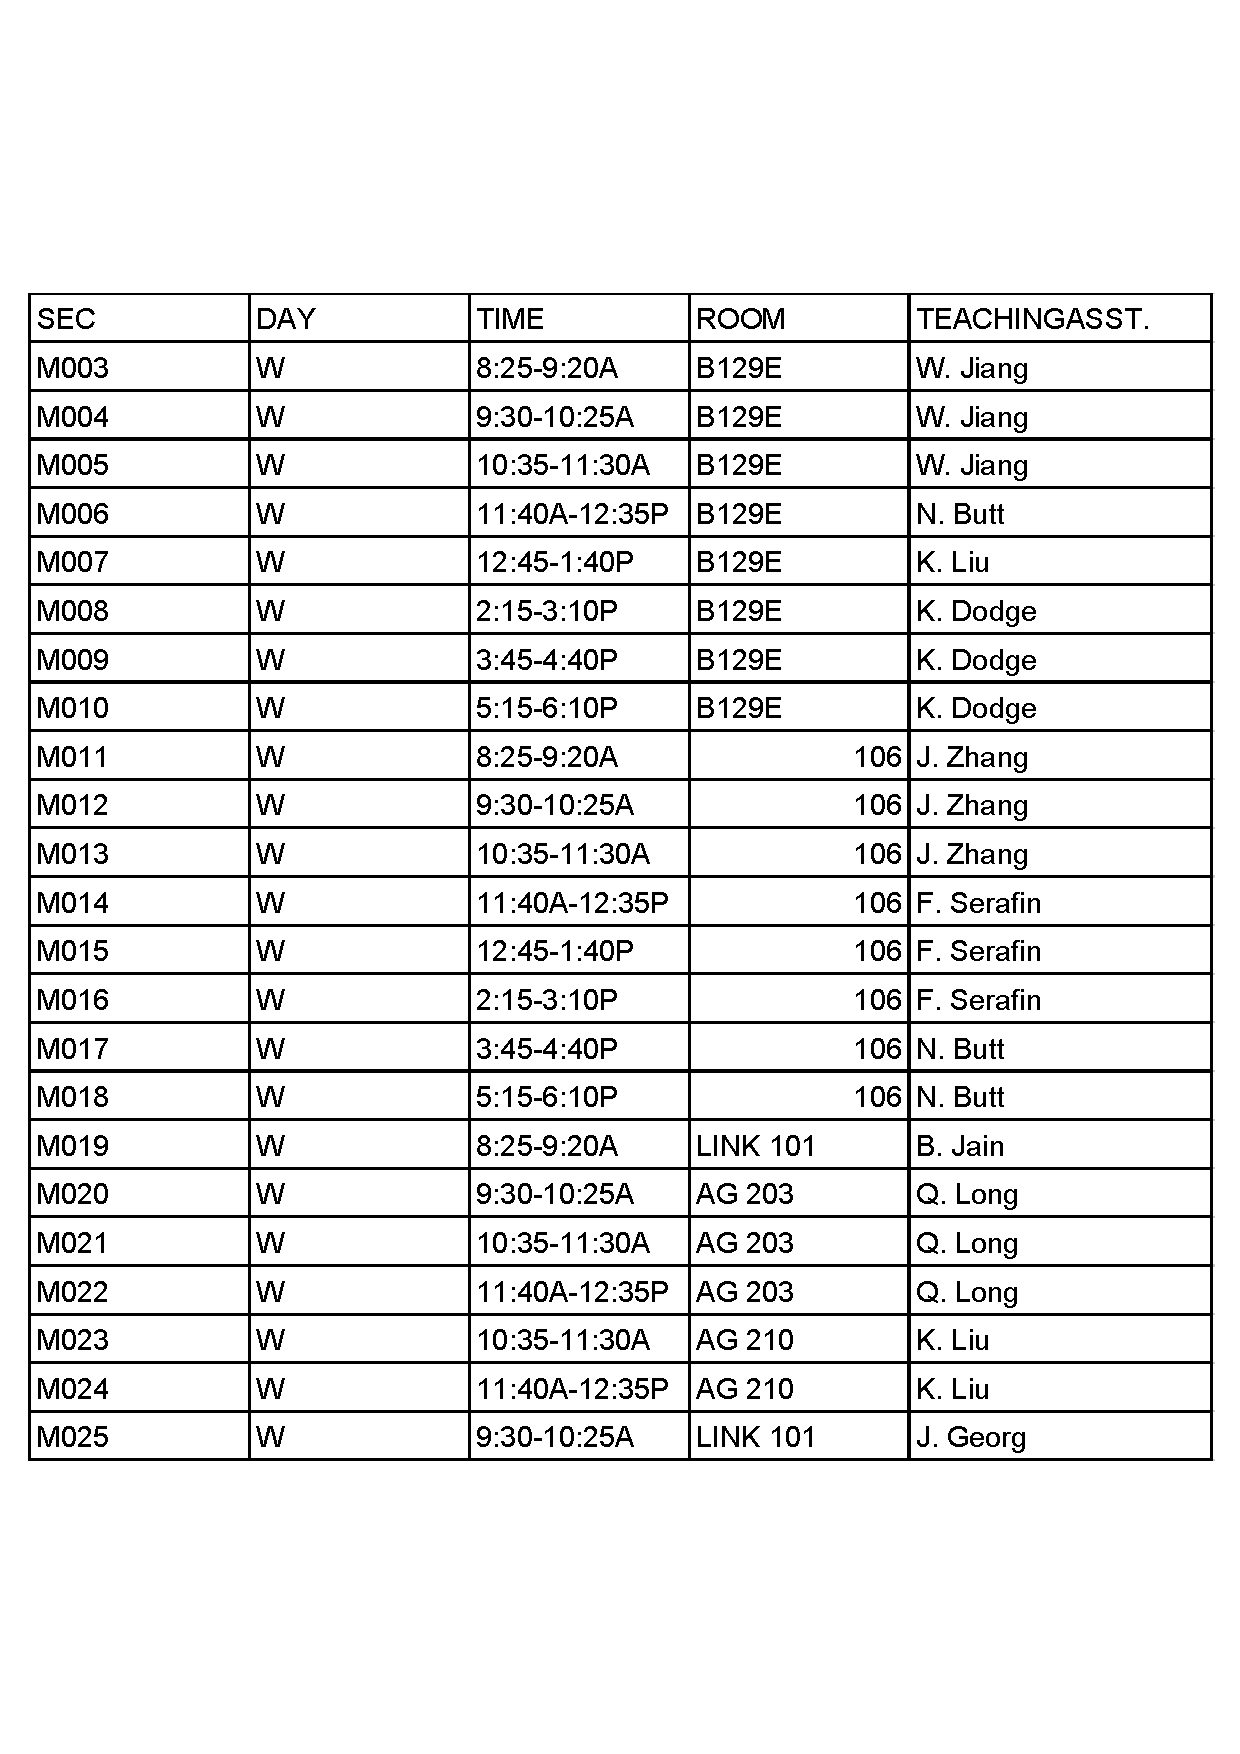
\includegraphics[width=0.9\textwidth]{sections.pdf}}

\newpage
\small





\begin{flushright}
    Name: \underline{\hspace{3in}}
    \end{flushright}
  
    \Large \centerline{\sc{Question 1}}
    \normalsize

  \rm

  A ``tire swing'' consists of an old tire of mass $M$ hanging from a light rope of length $L$, used as a playground toy by children. A child of mass $m$ runs and leaps onto the swing; when she 
  grabs the swing, she is moving horizontally with some unknown speed $v_0$. After she jumps onto the tire, it swings up into the air, reaching a maximum angle $\theta$.

  In this problem, you will determine the unknown speed $v_0$ in terms of $m$, $M$, $L$, $\theta$, and $g$.

  \it \bigskip 

  a) Describe a few sentences what happens in the different stages of the motion, and what physical principles you can use to understand each one. (You do not need to do any mathematics here.) (10 points)

  \bigskip

  \vspace{2in}

  b) Compute $v_0$ in terms of $m$, $M$, $L$, $\theta$, and $g$, showing any drawings that are helpful in your analysis. (15 points extra credit)

  \newpage


\newpage

\begin{flushright}
Name: \underline{\hspace{3in}}
        \end{flushright}

        \Large \centerline{\sc{Question 2}}
        \normalsize
        \rm

Merry and Pippin are sledding on the frozen surface of Lake Onondaga, which is quite close to a frictionless surface. Each of them plus his sled has a mass of 30 kg, but Merry also carries a stone that weighs 5 kg.
They are both traveling east at 2 m/s, right next to each other; Merry is north of Pippin. Merry throws his stone to Pippin, who catches it; the initial velocity of the stone is 5 m/s due south. Treat north as the positive $y-$axis and east as the 
positive $x-$axis.

\it \bigskip

a) What technique are you going to use to solve parts b and c? (3 points)

\vspace{0.3in}

b) What are the x and y components of Merry's velocity vector after he throws the stone? (6 points)

\vspace{1in}

c) What are the x and y components of Pippin's velocity vector after he catches the stone? (6 points)

\vspace{1in}

d) Initially, they had the same value of $v_x$. However, after one threw the stone and the other caught it, their $x-$velocities are different. Why is this? (Explain in words; no mathematics is required.) (5 points)

\vspace{1in}

e) Suppose that Merry threw the stone by holding it to his chest and pushing it outward with both hands, while Pippin had to reach behind him to catch it. After catching the stone, Pippin's sled begins to spin around. Why is this? (5 points)

\newpage


\begin{flushright}
Name: \underline{\hspace{3in}}
        \end{flushright}

        \Large \centerline{\sc{Question 3}}
        \normalsize
        \rm

        Answer the following questions with ``sometimes'', ``always'', or ``never''. \it (2.5 points each)

\it \bigskip

a) Momentum is conserved in a partially inelastic collision.

\bigskip

b) If a spring's potential energy increases, then some other force did positive work on the spring.

\bigskip

c) If an object is rotating, then the torque around its center of mass is zero.

\bigskip

d) If an object rolls without slipping, then its angular velocity is equal to its translational (center-of-mass) velocity.

\bigskip

e) If a uniform solid sphere and a ring roll down a hill from rest, the sphere will roll faster. (Note that the radii and masses may differ. Ignore friction and drag.)

\bigskip

f) If a 10 N and a 20 N force are applied to the same point on an object, the 20 N force will create a greater torque. 

\bigskip

g) When an object moves in two dimensions, it is necessary to examine the conservation of energy separately in $x$ and $y$.

\bigskip

h) The torque (about the center) applied by a centripetal force is positive.

\bigskip

i) If an object of mass 1 kg moving at 4 m/s collides and sticks to an object of mass 2 kg moving at 1 m/s, the combination will be moving at 2 m/s after the collision.

\bigskip

j) Angular momentum is conserved if there are no external torques.


\newpage


\begin{flushright}
Name: \underline{\hspace{3in}}
        \end{flushright}

\begin{minipage}[b]{0.4\textwidth}
  \small
  \vspace{-0.8in}
A 4m-long pole of mass 80 kg extends from the side of a building, angled at 60 degrees above the horizontal. One meter from the end of the pole, a sign of mass 50 kg is attached. To support the pole,
a horizontal cable runs from the end of the pole to the building. (See the attached figure.)

\bigskip
\bigskip

\end{minipage}
\begin{minipage}[t]{0.6\textwidth}
  \begin{flushright}
  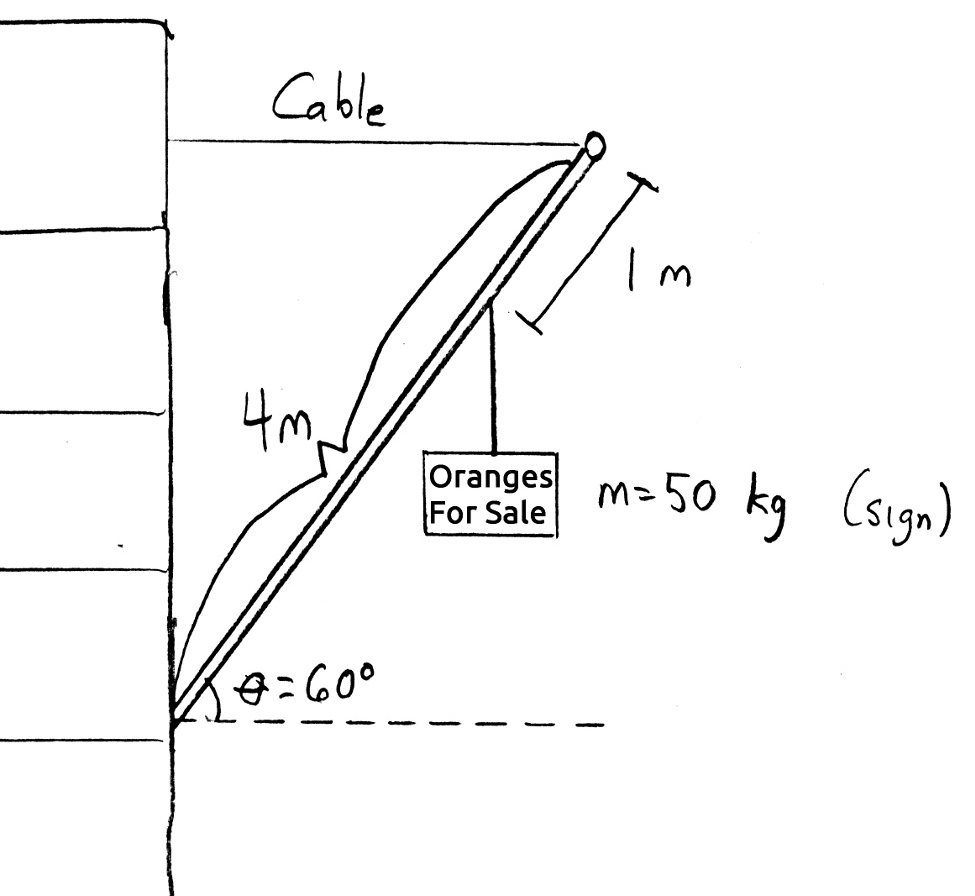
\includegraphics[width=0.9\textwidth]{sign2.jpg}
\end{flushright}
\end{minipage}

\bigskip
\bigskip

\it

a) Draw a force diagram on the back of this page, showing all of the elements needed to help you compute the tension in the support cable. Indicate 
your choice of pivot point. (5 points)

\bigskip

b) Compute the tension in the cable. (15 points)

\vspace{2 in}

c) Suppose now that the store owner wanted to attach the cable to a different point on the building in order to minimize its tension. What angle between the 
cable and the horizontal would support the pole with the minimum tension? (5 points)
\newpage


\Large \centerline{\sc{Question 5}}
\rm
\normalsize
A mischievous cat knocks a spool of yarn of mass $m$ and radius $r$ off of a table, which you may model as a uniform cylinder ($I=\frac{1}{2}mr^2$). The cat holds one end of the yarn as it falls, so the spool unrolls as it falls. In this problem,
you will compute the acceleration of the spool.

\bigskip
\bigskip

\it

a) Draw a force diagram for the spool on the back of this page, showing all elements that will help you solve the problem. Indicate your choice of coordinate system. (5 points)

\bigskip

b) What mathematical expression relates its angular acceleration to its linear acceleration? (3 points)

\vspace{1in}

c) In terms of $m$, $g$, and $r$, calculate the acceleration of the falling spool of yarn. (Your answer may not depend on all three quantities.) (10 points)

\vspace{2.5in}

d) If the spool consisted of yarn wrapped around an iron bar, but with the same total mass, would the acceleration increase, decrease, or stay the same? Why? (3 points)

\vspace{0.5in}

e) If the spool consisted of yarn wrapped around a thin cardboard tube, but with the same total mass, would the acceleration increase, decrease, or stay the same? Why? (3 points)



\newpage
\Large\centerline{\sc{Scratch Paper for Problem \underline{\hspace{1in}}}}
\newpage
\Large\centerline{\sc{Scratch Paper for Problem \underline{\hspace{1in}}}}
\newpage





\Large \centerline{\sc Reference Sheet}

\normalsize \rm

Centripetal acceleration of an object in uniform circular motion: $a_c = \frac{v_T^2}{r}\,\, {\rm{or}}\,\, \omega^2 r$

\bigskip

Tangential velocity $v_T = \omega r$\\
Tangential acceleration $a_T = \alpha r$

\bigskip

Newton's second law: $\vec F = m \vec a$ \\
Newton's third law: $\vec F_{\rm{A\, on\, B}} = -\vec F_{\rm{ B\, on\, A}}$

\bigskip

Momentum $\vec p=m \vec v$

\bigskip

Maximum force of static friction: $\mu_s F_N$ \\
Force of kinetic friction: $\mu_s F_N$

\bigskip

\centerline{  \begin{tabular}{| c | c |}
      \hline
      Translation & Rotation \\
      \hline
      \hline
      \hline
      Position $x$ & Angle $\theta$ \\
      \hline
      Velocity $v$ & Angular velocity $\omega$ \\
      \hline
      Acceleration $a$ & Angular acceleration $\alpha$ \\
      \hline
      \hline
      $v(t) = v_0 + at$ & $\omega(t) = \omega_0 + \alpha t$ \\
      \hline
      $x(t) = x_0 + v_0 t + \frac{1}{2}at^2$ & $\theta(t) = \theta_0 + \omega_0 t + \frac{1}{2} \alpha t^2$ \\
      \hline
      $v_f^2 - v_0^2 = 2a \Delta x$ & $ \omega_f^2 - \omega_0^2 = 2 \alpha \Delta \theta$ \\
      \hline
      \hline
      Force $\vec F$ & Torque: $\tau=F_\perp r$ or $F r_\perp$\\
      \hline
      Mass $m$ & Moment of Inertia: $I = \lambda MR^2$ \\
      \hline
      \hline
      Newton's second law $\vec F = m \vec a$ & Newton's second law for rotation $\tau = I \alpha$ \\
      \hline
      \hline
      Work = $\vec F \cdot \Delta \vec s$ & Work = $\tau \Delta \theta$ \\
      \hline
      Kinetic energy $\frac{1}{2} mv^2$ & Kinetic energy $\frac{1}{2} I \omega^2$ \\
      \hline
      Power ($\vec F$ constant) = $\vec F \cdot \vec v$ & Power ($\tau$ constant) = $\tau \omega$ \\
      \hline
      \hline
      Momentum $\vec p = m \vec v$ & Angular momentum $L = I \omega$ \\
      \hline
  \end{tabular}}
  Moment of inertia of...

  \begin{itemize}
    \item{Any object: $I=m \LL r^2 \RR$, where $\LL r^2 \RR$ is the average squared radius}
    \item{A hollow cylinder or single mass a distance $r$ from the pivot: $I=mr^2$}
    \item{A solid sphere: $I=\frac{2}{5}mr^2$}
    \item{A cylinder or disk: $I=\frac{1}{2}mr^2$}
  \end{itemize}

\bigskip

Angular momentum of a single object about a pivot: $L = mvr_\perp = m v_\perp r$


\end{document}
